%%%%%%%%%%%%%%%%%%%%%%%%%%%%%%%%%%%%%%%
% Wenneker Resume/CV
% LaTeX Template
% Version 1.1 (19/6/2016)
%
% This template has been downloaded from:
% http://www.LaTeXTemplates.com
%
% Original author:
% Frits Wenneker (http://www.howtotex.com) with extensive modifications by 
% Vel (vel@LaTeXTemplates.com)
%
% License:
% CC BY-NC-SA 3.0 (http://creativecommons.org/licenses/by-nc-sa/3.0/
%
%%%%%%%%%%%%%%%%%%%%%%%%%%%%%%%%%%%%%%

%----------------------------------------------------------------------------------------
%	PACKAGES AND OTHER DOCUMENT CONFIGURATIONS
%----------------------------------------------------------------------------------------

\documentclass[a4paper,12pt]{memoir} % Font and paper size
\usepackage{lipsum}
\usepackage{nicefrac}

%%%%%%%%%%%%%%%%%%%%%%%%%%%%%%%%%%%%%%%%%
% Wenneker Resume/CV
% Structure Specification File
% Version 1.1 (19/6/2016)
%
% This file has been downloaded from:
% http://www.LaTeXTemplates.com
%
% Original author:
% Frits Wenneker (http://www.howtotex.com) with extensive modifications by 
% Vel (vel@latextemplates.com)
%
% License:
% CC BY-NC-SA 3.0 (http://creativecommons.org/licenses/by-nc-sa/3.0/)
%
%%%%%%%%%%%%%%%%%%%%%%%%%%%%%%%%%%%%%%%%%

%----------------------------------------------------------------------------------------
%	PACKAGES AND OTHER DOCUMENT CONFIGURATIONS
%----------------------------------------------------------------------------------------

\usepackage{XCharter} % Use the Bitstream Charter font
\usepackage[utf8]{inputenc} % Required for inputting international characters
\usepackage[T1]{fontenc} % Output font encoding for international characters

\usepackage[top=1cm,left=1cm,right=1cm,bottom=1cm]{geometry} % Modify margins

\usepackage{graphicx} % Required for figures

\usepackage{flowfram} % Required for the multi-column layout

\usepackage{url} % URLs

\usepackage[usenames,dvipsnames]{xcolor} % Required for custom colours

\usepackage{tikz} % Required for the horizontal rule

\usepackage{enumitem} % Required for modifying lists
\setlist{noitemsep,nolistsep} % Remove spacing within and around lists

\setlength{\columnsep}{\baselineskip} % Set the spacing between columns

% Define the left frame (sidebar)
\newflowframe{0.2\textwidth}{\textheight}{0pt}{0pt}[left]
\newlength{\LeftMainSep}
\setlength{\LeftMainSep}{0.2\textwidth}
\addtolength{\LeftMainSep}{1\columnsep}
 
% Small static frame for the vertical line
\newstaticframe{1.5pt}{\textheight}{\LeftMainSep}{0pt}
 
% Content of the static frame with the vertical line
\begin{staticcontents}{1}
\hfill
\tikz{\draw[loosely dotted,color=RoyalBlue,line width=1.5pt,yshift=0](0,0) -- (0,\textheight);}
\hfill\mbox{}
\end{staticcontents}
 
% Define the right frame (main body)
\addtolength{\LeftMainSep}{1.5pt}
\addtolength{\LeftMainSep}{1\columnsep}
\newflowframe{0.7\textwidth}{\textheight}{\LeftMainSep}{0pt}[main01]

\pagestyle{empty} % Disable all page numbering

\setlength{\parindent}{0pt} % Stop paragraph indentation

%----------------------------------------------------------------------------------------
%	NEW COMMANDS
%----------------------------------------------------------------------------------------

\newcommand{\userinformation}[1]{\renewcommand{\userinformation}{#1}} % Define a new command for the CV user's information that goes into the left column

\newcommand{\cvheading}[1]{{\Huge\bfseries\color{RoyalBlue} #1} \par\vspace{.6\baselineskip}} % New command for the CV heading
\newcommand{\cvsubheading}[1]{{\Large\bfseries #1} \bigbreak} % New command for the CV subheading

\newcommand{\Sep}{\vspace{1em}} % New command for the spacing between headings
\newcommand{\SmallSep}{\vspace{0.5em}} % New command for the spacing within headings

\newcommand{\aboutme}[2]{ % New command for the about me section
\textbf{\color{RoyalBlue} #1}~~#2\par\Sep
}
	
\newcommand{\CVSection}[1]{ % New command for the headings within sections
{\Large\textbf{#1}}\par
\SmallSep % Used for spacing
}

\newcommand{\CVItem}[2]{ % New command for the item descriptions
\textbf{\color{RoyalBlue} #1}\par
#2
\SmallSep % Used for spacing
}

\newcommand{\bluebullet}{\textcolor{RoyalBlue}{$\circ$}~~} % New command for the blue bullets
 % Include the file specifying document layout and packages

%----------------------------------------------------------------------------------------
%	NAME AND CONTACT INFORMATION 
%----------------------------------------------------------------------------------------

\userinformation{ % Set the content that goes into the sidebar of each page
\begin{flushright}
% Comment out this figure block if you don't want a photo
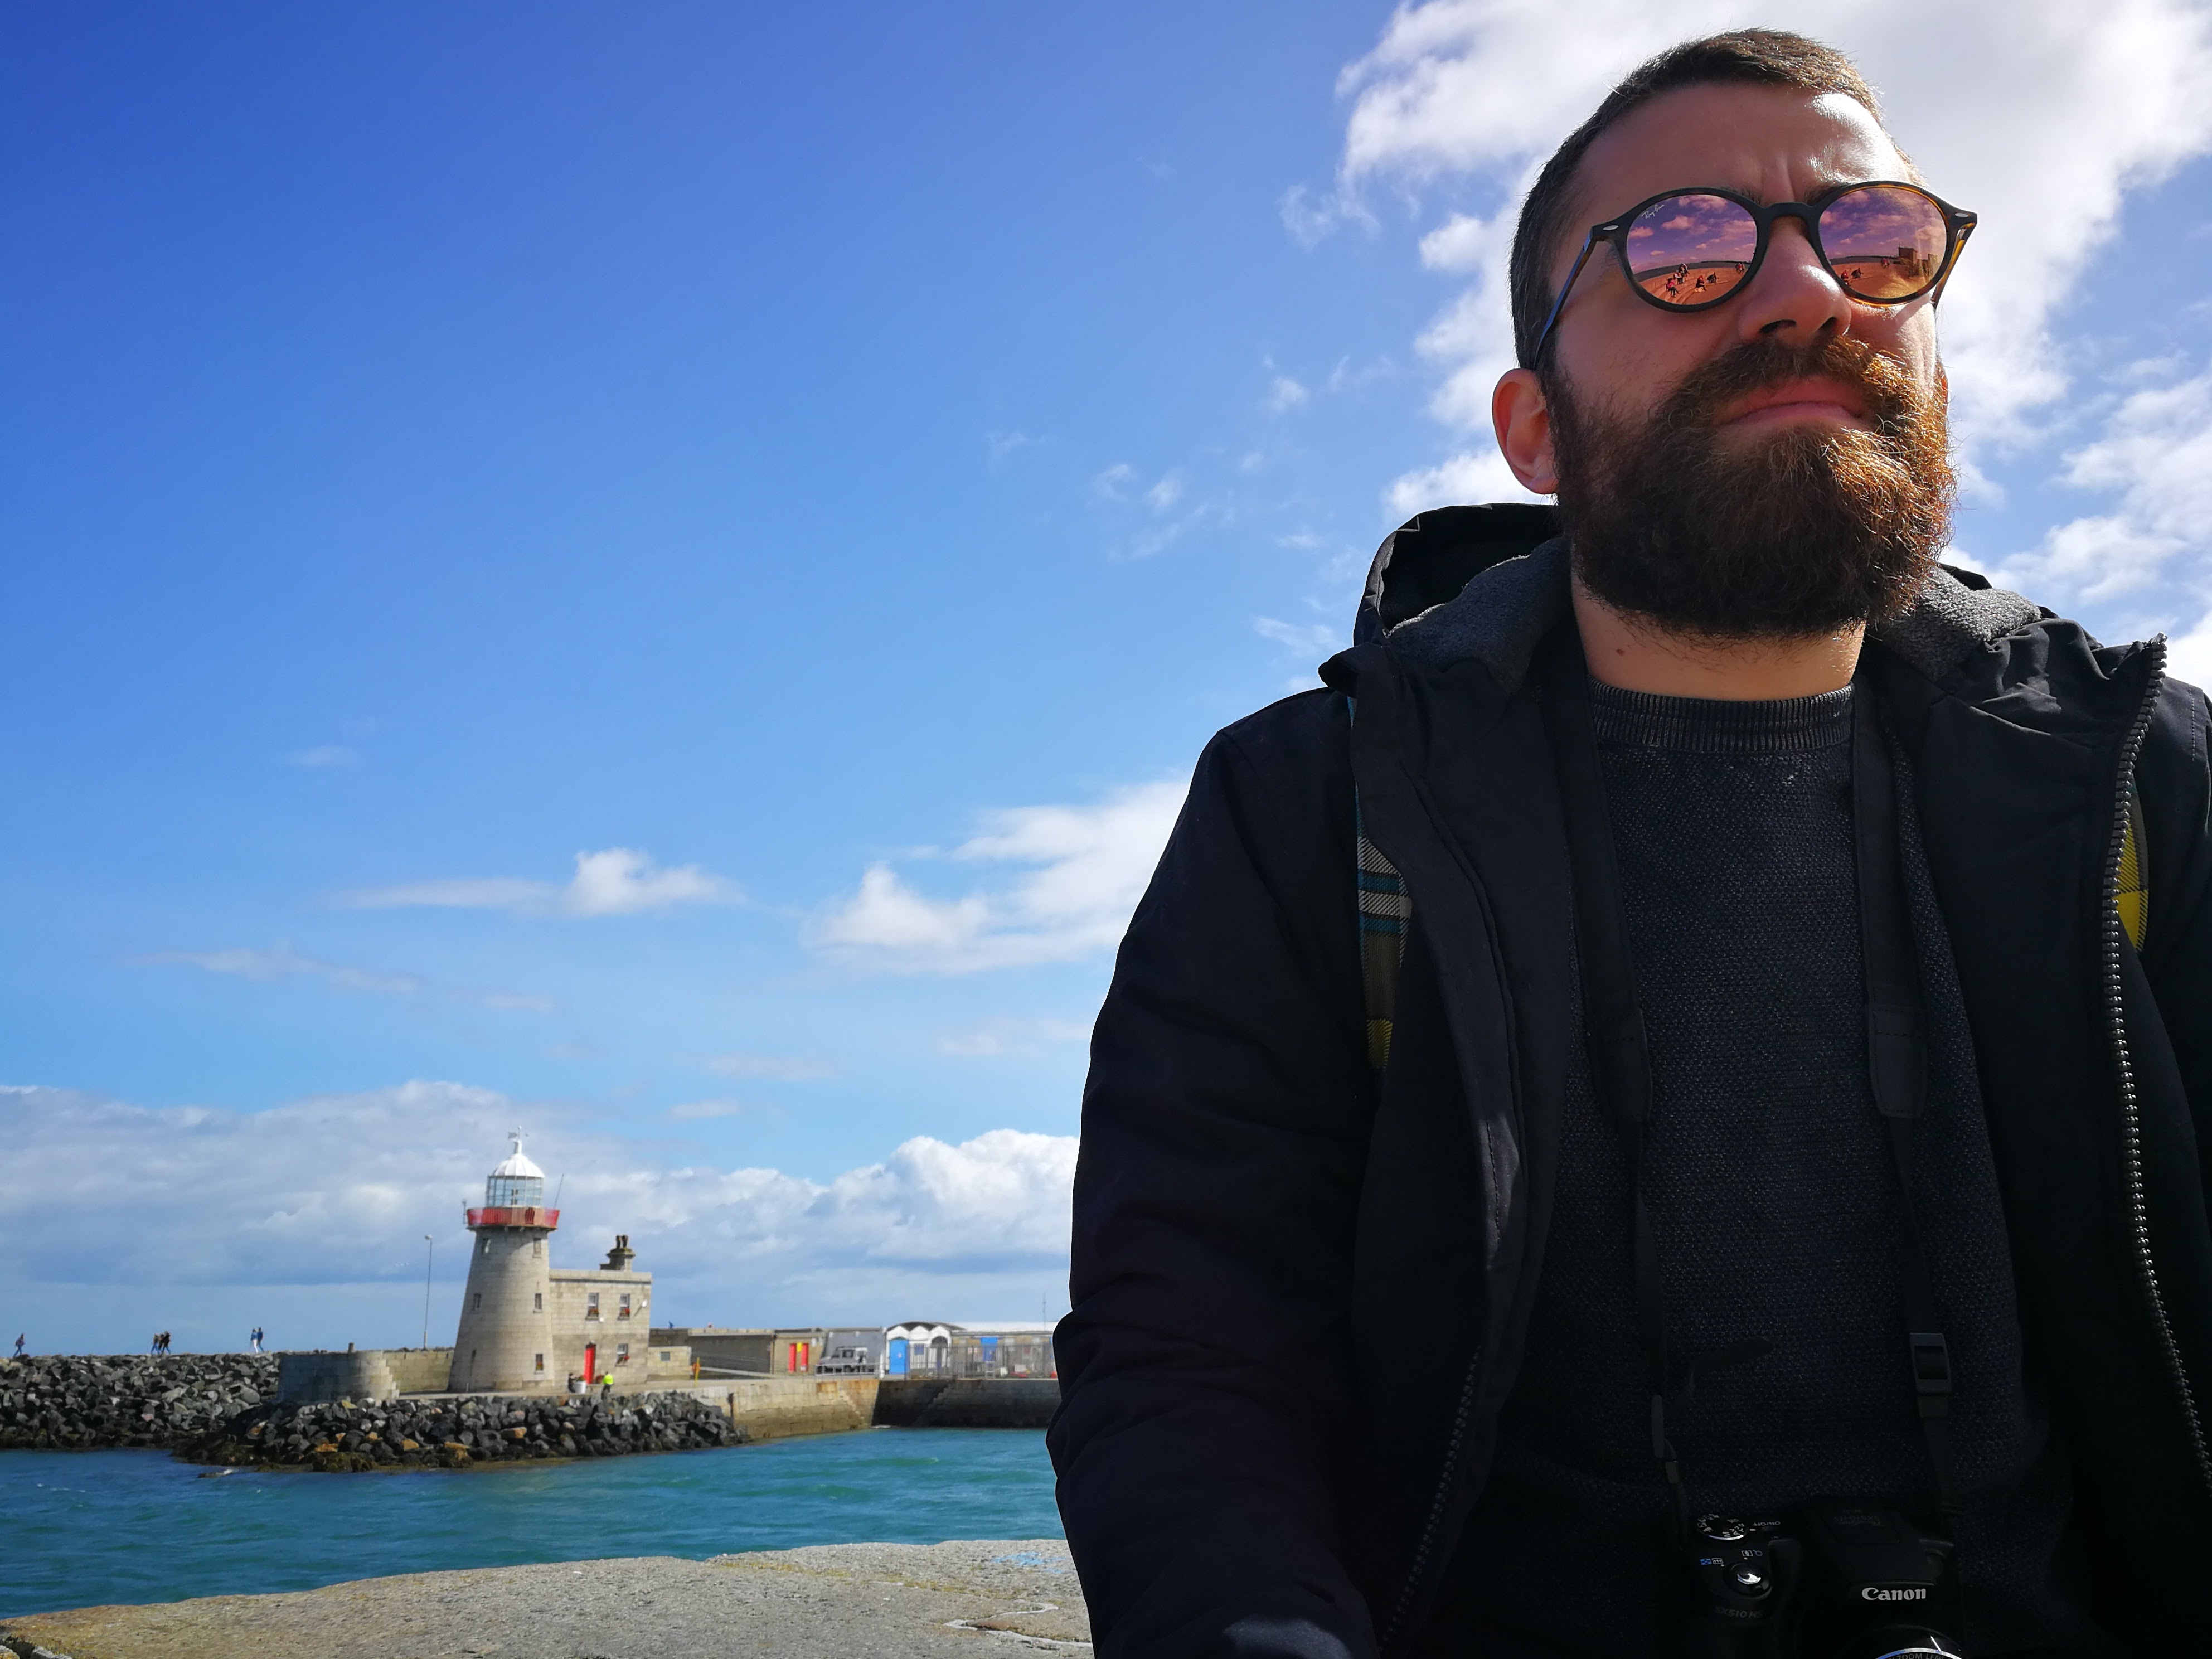
\includegraphics[width=0.9\columnwidth]{media/me0.jpg}\\[\baselineskip] % Your photo
\small % Smaller font size
\textbf{Mail} \\
\textit{ialoise@diag.uniroma1.it} \\ % Your email address
\Sep

\textbf{Personal Site}\\
\textit{https://goo.gl/85uhCK}\\
\Sep

\textbf{LinkedIn} \\
\textit{https://goo.gl/NQvHbJ} \\ % Your URL
\Sep

\textbf{Birthday} \\
21 Maggio 1991
\vfill % Whitespace under this block to push it up under the photo
\end{flushright}
}

%----------------------------------------------------------------------------------------

\begin{document}

\userinformation % Print your information in the left column

\framebreak % End of the first column

%----------------------------------------------------------------------------------------
%	HEADING
%----------------------------------------------------------------------------------------

\cvheading{Irvin Aloise} % Large heading - your name

\cvsubheading{Software Engineer} % Subheading - your occupation/specialization

%----------------------------------------------------------------------------------------
%	ABOUT ME
%----------------------------------------------------------------------------------------

% \aboutme{About Me}{\lipsum[1]}

%----------------------------------------------------------------------------------------
%	EDUCATION
%----------------------------------------------------------------------------------------

\CVSection{Education}

%------------------------------------------------

\CVItem{2017 - now, Sapienza University of Rome}{\textbf{Ph.D. in Computer Science} (in English) \\
    Research Topics: Mobile Robotics, Simultaneous Localization and Mapping, Computer Vision.\\
    Supervisor: \textit{Prof. Giorgio Grisetti}}


%------------------------------------------------

\CVItem{2014 - 2017, Sapienza University of Rome}{\textbf{Master of Science in Artificial Intelligence and Robotics} (in English) \\
Thesis title: \textit{Extended Measurements in Pose-Graph Optimization} \\
Supervisor: \textit{Prof. Giorgio Grisetti} and \textit{Ph.D. Dominik Schlegel} \\
Final grades: First Class with Honors ($\nicefrac{110}{110}$ cum laude)}

%------------------------------------------------

\CVItem{2010 - 2014, Sapienza University of Rome}{\textbf{Bachelor of Science in Electronic Engineering} (in Italian) \\
Thesis title: \textit{L'uso del Capture Point nello studio della reazione alle spinte nei robot umanoidi}. \\
Supervisor: \textit{Prof. Giuseppe Oriolo} \\
Final grades: $\nicefrac{100}{110}$}

%------------------------------------------------

\Sep % Extra whitespace after the end of a major section
\Sep % Extra whitespace after the end of a major section

%------------------------------------------------

%----------------------------------------------------------------------------------------
%	PUBLICATIONS
%----------------------------------------------------------------------------------------

\CVSection{Publications}

%------------------------------------------------


\CVItem{Sep 2018}{
\textbf{Matrix Difference in Pose-Graph Optimization} \\
Pose-Graph optimization is a crucial component of many modern SLAM systems. Most prominent state of the art systems address this problem by iterative non-linear least squares. Both number of iterations and convergence basin of these approaches depend on the error functions used to describe the problem. The smoother and more convex the error function with respect to perturbations of the state variables, the better the least-squares solver will perform. In this paper we propose an alternative error function obtained by removing some non-linearities from the standard used one - i.e. the geodesic error function -  that exhibits a larger convergence basin.}


%------------------------------------------------

\Sep % Extra whitespace after the end of a major section
\Sep % Extra whitespace after the end of a major section

%----------------------------------------------------------------------------------------
%	PERSONAL PROJECTS
%----------------------------------------------------------------------------------------

\CVSection{Personal Projects}

%------------------------------------------------

\CVItem{Nov 2016 - Feb 2017, Sapienza Univesity of Rome, Exam project}{
\textbf{Person Detection and Tracking for Human-Robot Interaction} \\
This project aims to detect and track a person in human-friendly environments (like in a school). The system is developed for a differential drive robot and exploits laser data together with RGB-D images to achieve the goal. It has been developed a ROS package that uses \textit{OpenCV} to perform proper image processing in an efficient way.}

%----------------------------------------------------------------------------------------
%   NEW PAGE
%----------------------------------------------------------------------------------------
%------------------------------------------------
\clearpage % Start a new page
\userinformation % Print your information in the left column
\framebreak % End of the first column

\CVItem{Jul 2016 - Dec 2016, Sapienza Univesity of Rome, Exam project}{
\textbf{Development of a Simulation Environment for Teleoperated Surgical Task} \\
Realization of a simulative framework for a teleoperation task between a real haptic device (Geomagic Touch) and a virtual manipulator (KUKA LBR 4+) using VREP software. The surgical task that has been designed is a needle penetration in a simulated biological tissue.}

\CVItem{Jun 2016 - Jul 2016, Sapienza University of Rome, Exam project}{
\textbf{Analyzing Visualization Techniques for Convolutional Neural Neworks} \\ 
In this project, it has been tested and reproduced some of the most employed visualization
techniques for Convolutional Neural Networks (CNNs), in order to better understand the representation of the images that a network produces. This has been developed using the \textit{Caffe} framework.}

%------------------------------------------------

\CVItem{Oct 2015 - Dec 2015, Sapienza University of Rome, Exam project}{
\textbf{MIDI Classification Using Similarity Metric Based on Kolmogorov Complexity} \\
The project proposes a method to classify MIDI instances by author, evaluating a similarity metric based on the concept of Kolmogorov Complexity. The classifier can be used as the first stage of a multi-stage classifier, in order to bias more specific units. 
The entire project has been developed in \textit{MATLAB}.}

\CVItem{Dec 2014 - Feb 2015, Sapienza University of Rome, Exam project}{
\textbf{A Third Person Game Based on the Three.js Library} \\
It has been developed a game based on WebGL using a Javascript library 
(\textit{Three.js}). The game is straightforward and it can be played on a browser 
that supports HTML5.}

\Sep
\Sep

%----------------------------------------------------------------------------------------
%	TEACHING
%----------------------------------------------------------------------------------------

\CVSection{Teaching Activities}

\CVItem{Sep 2018 - June 2019, Sapienza University of Rome}{\textbf{Tutoring for the course of \textit{Sistemi 
      Operativi}}\\ The course is within the B.Sc. in Computer Science, 6 ECTS credits.}

\Sep

\CVItem{Nov 2017 - Feb 2018, Sapienza University of Rome}{\textbf{Tutoring for the course of \textit{Sistemi 
      Operativi}}\\ The course is within the B.Sc. in Computer Science, 6 ECTS  credits.}
\Sep
\Sep

%----------------------------------------------------------------------------------------
%	SKILLS
%----------------------------------------------------------------------------------------

\CVSection{Computer Skills}

%------------------------------------------------

\CVItem{Programming}
{\begin{tabular}{p{0.2\textwidth} p{0.2\textwidth} p{0.2\textwidth}}
\bluebullet C++ &  \bluebullet Matlab & \bluebullet Python\\
\bluebullet C &  \bluebullet HTML & \bluebullet Javascript\\
\bluebullet \LaTeX
\end{tabular}}

%------------------------------------------------

\CVItem{Other Software}
{\begin{tabular}{p{0.2\textwidth} p{0.2\textwidth} p{0.2\textwidth}}
 \bluebullet OpenCV &  \bluebullet ROS & \bluebullet OpenGL \\
\end{tabular}}

%------------------------------------------------

\CVItem{Operating Systems}
{\begin{tabular}{p{0.2\textwidth} p{0.2\textwidth} p{0.2\textwidth}}
\bluebullet Ubuntu &  \bluebullet Windows & \bluebullet MacOS \\
\end{tabular}}

%------------------------------------------------

\Sep % Extra whitespace after the end of a major section

%----------------------------------------------------------------------------------------
%	AWARDS
%----------------------------------------------------------------------------------------

%----------------------------------------------------------------------------------------
%   NEW PAGE
%----------------------------------------------------------------------------------------
%------------------------------------------------
\clearpage % Start a new page
\userinformation % Print your information in the left column
\framebreak % End of the first column
\CVSection{Languages}

%------------------------------------------------

\CVItem{Italian}{Mother-tongue}

%------------------------------------------------

\CVItem{English}{Advanced}

%------------------------------------------------

\Sep % Extra whitespace after the end of a major section
\Sep % Extra whitespace after the end of a major section

%----------------------------------------------------------------------------------------
%	INTERESTS
%----------------------------------------------------------------------------------------

\CVSection{Interests}

%------------------------------------------------

\CVItem{Professional}{Robotics, SLAM, Machine Learning, Deep Learning, Convolutional Neural Networks, Computer Vision, Autonomous Robotics}

%------------------------------------------------

\CVItem{Personal}{Music, photography, cinema, technology, motor sports}

%------------------------------------------------

\Sep % Extra whitespace after the end of a major section

%----------------------------------------------------------------------------------------

\end{document}
